    \documentclass[../CSC_5RO06_TA.tex]{subfiles}

\begin{document}
\section*{Question 4}

\subsection{Création des IP's Integrator}

Après la mise en œuvre d'une première configuration d'un accélérateur matériel de multiplication de matrices, un algorithme TCL a été conçu afin que diverses configurations puissent être générées automatiquement.

Dans cette implémentation, un même fichier contenait tous les différents algorithmes dans un même ensemble de fichiers, lesquels étaient sélectionnés lors de la création du projet en passant comme argument pour l'importation de fichiers le flag flag\_importation. Cela permettait la compilation d'un fichier avec uniquement la structure nécessaire et rien de plus.

De plus, cette configuration a garanti que la même structure de simulation soit maintenue au cours des différentes simulations, assurant ainsi la comparabilité des résultats. En outre, cela a permis d'exécuter des simulations avec des tailles de matrices arbitraires, offrant une grande flexibilité dans le choix des algorithmes. Lors de l'exécution, un patch correctif de Vivado HLS a été nécessaire pour corriger un bug du système.

Par la suite, un algorithme en Python a été développé pour effectuer l'extraction automatique des informations des rapports de synthèse de chaque configuration et les enregistrer dans un fichier CSV, qui serait ensuite utilisé pour générer les graphiques nécessaires afin de présenter les résultats obtenus. Ci-dessous se trouve le graphique avec les résultats de la multiplication naïve de matrices.
\begin{figure}[H]
    \centering
    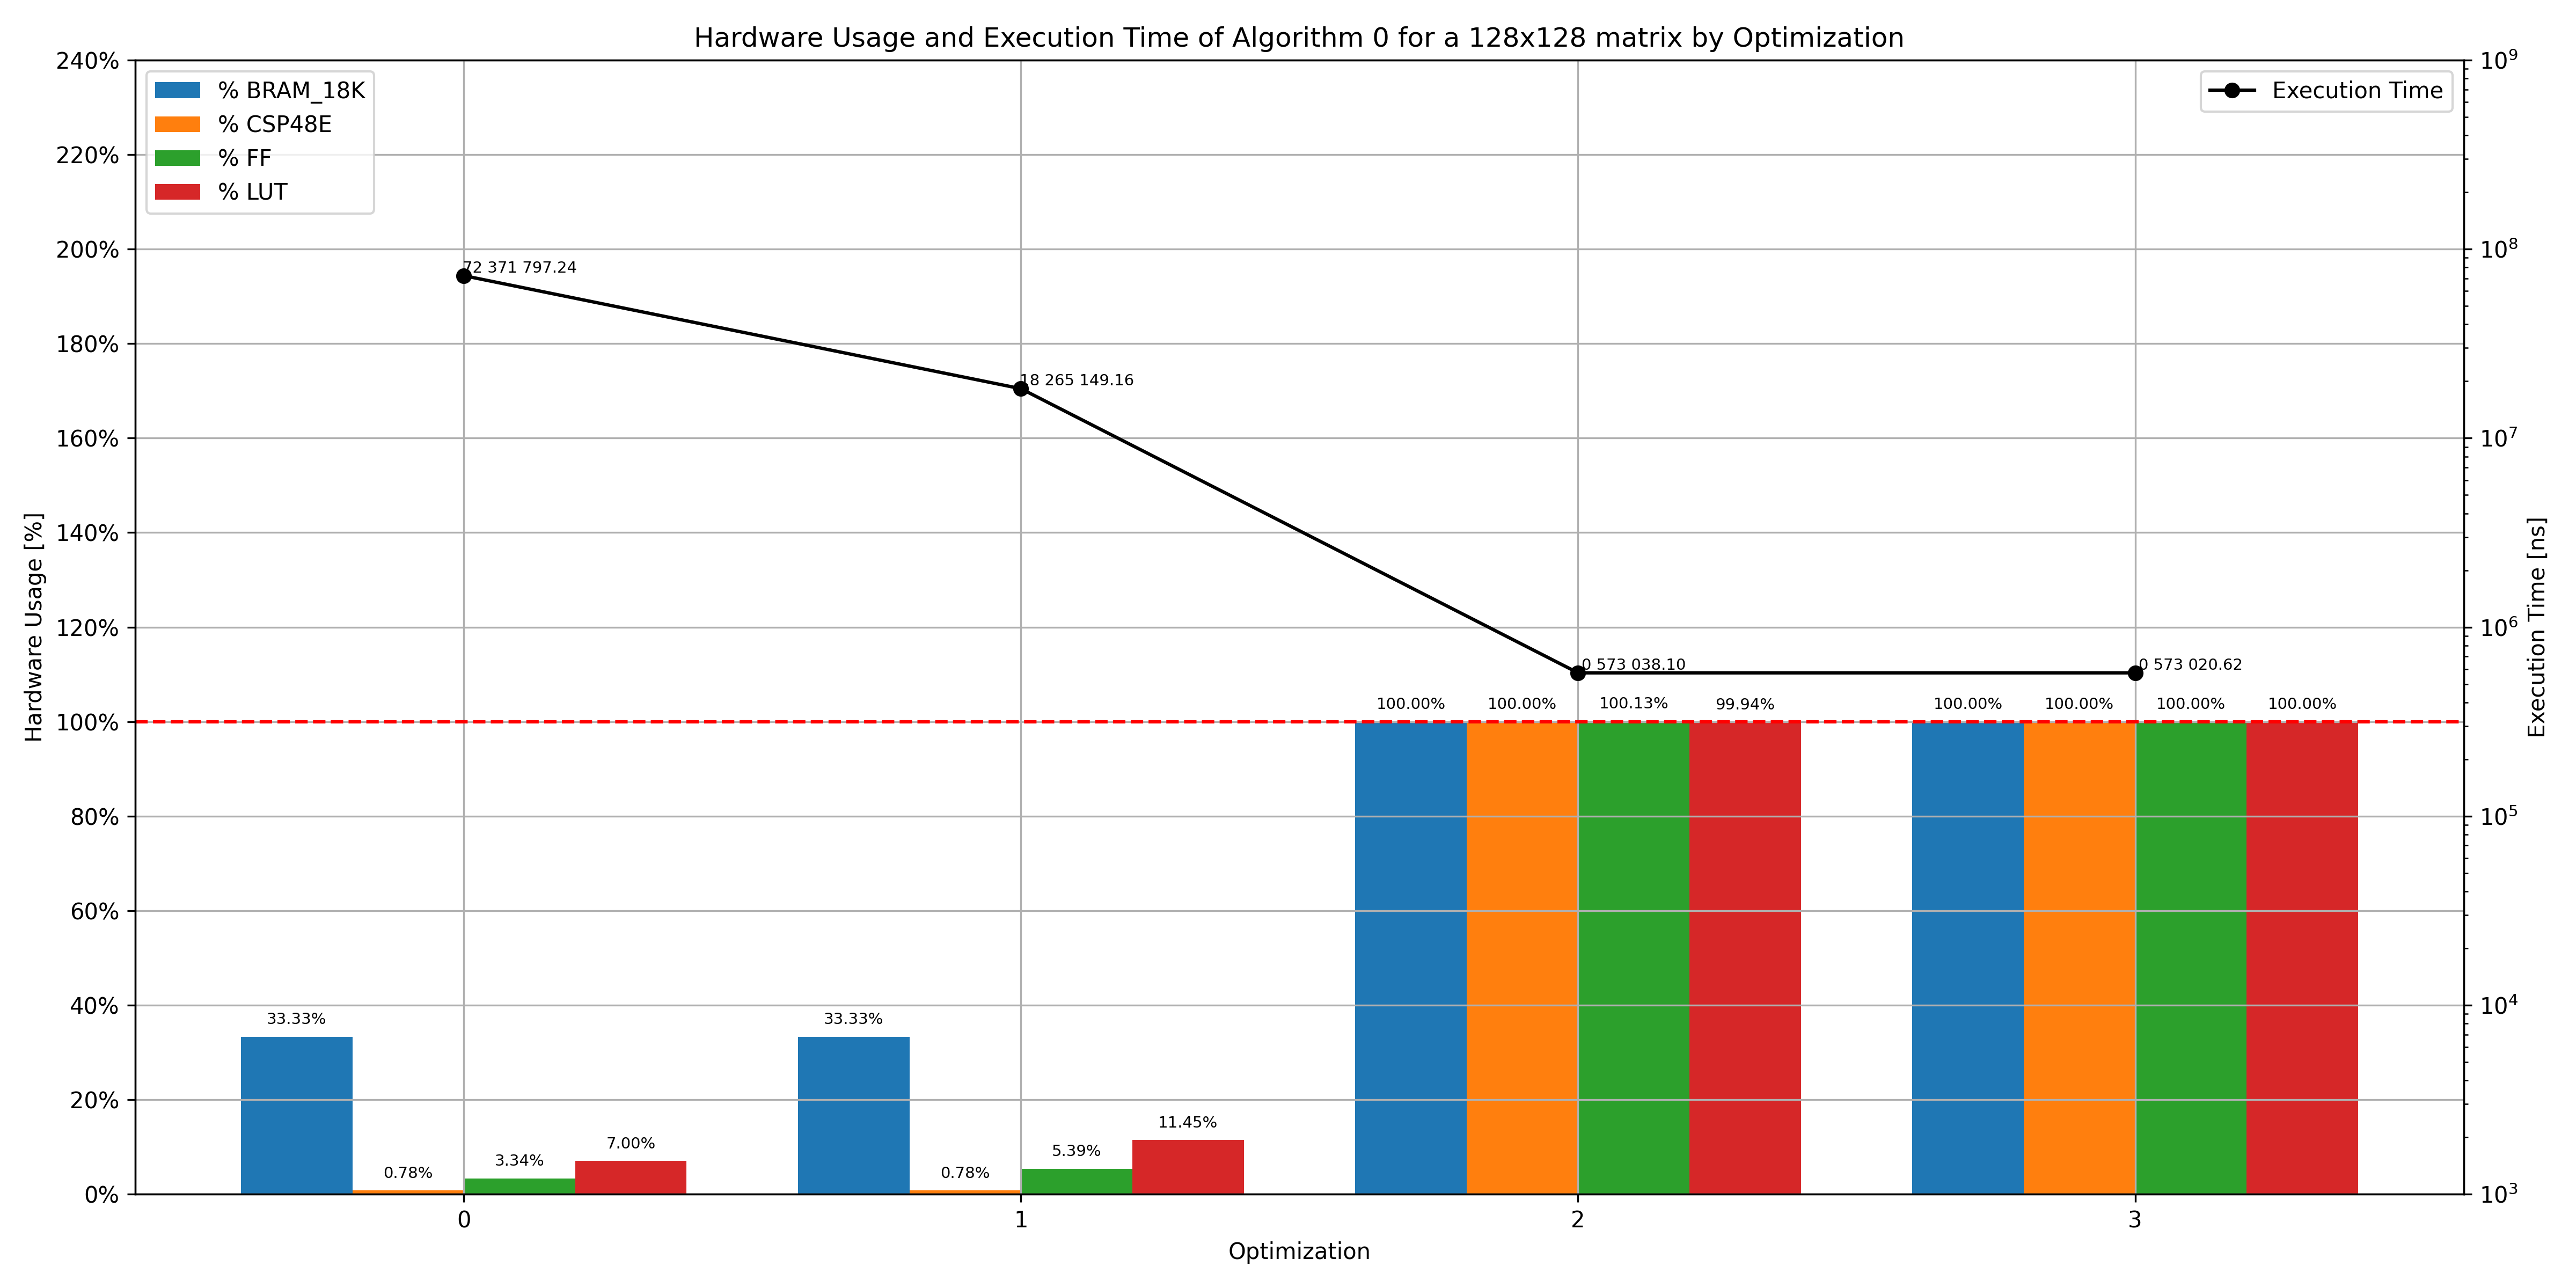
\includegraphics[width=1\columnwidth]{Images/hardware_usage_optimization_0_128.png}
    \caption{Naïve Algorithme par Optimisation}
\end{figure}

Même si, dans cette simulation, l'utilisation des ressources physiques du système était théoriquement optimale en utilisant toutes les ressources disponibles, en pratique, ce circuit ne peut pas être implémenté.

\subsection{Mettre en Oeuvre sur Vivado}

Une fois générés, l'algorithme HLS produisait les IPs nécessaires utilisés dans la représentation du Block Diagram pour synthétiser le circuit à implémenter sur la carte ZedBoard:

\begin{figure}[H]
    \centering
    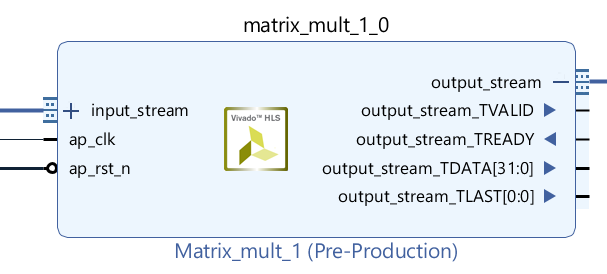
\includegraphics[width=1\columnwidth]{Images/IP.png}
    \caption{IP crée}
\end{figure}

Lorsqu'il est mis en œuvre dans la conception par blocs, le circuit final reliant les autres dispositifs est le suivant :


\begin{figure}[H]
    \centering
    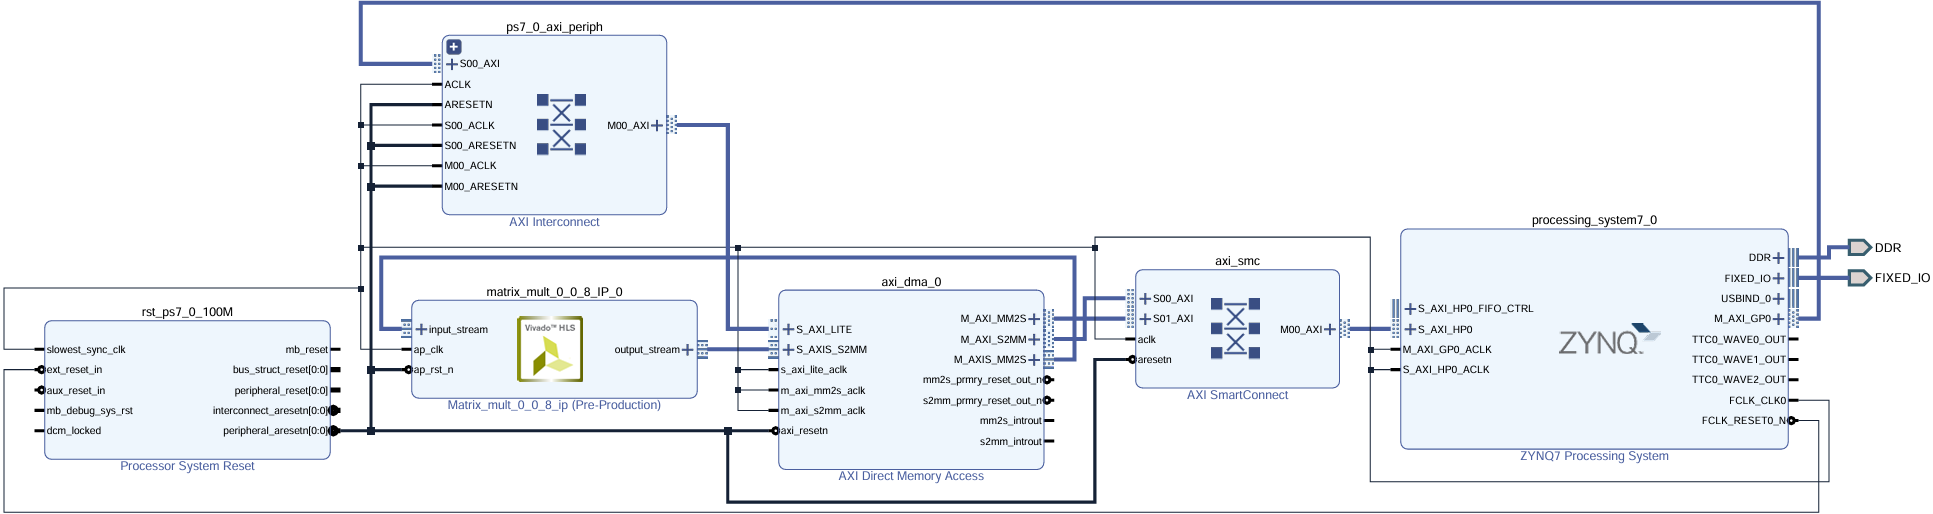
\includegraphics[width=1\columnwidth]{Images/vivado_HLS_implementation.png}
    \caption{Diagrame Block Design sur Vivado}
\end{figure}

Dans ce cas, il s'agit de la représentation du Block Diagram responsable de l'algorithme naïf, sans optimisation pour une matrice de taille 16 x 16. Toutefois, la structure du diagramme ne changera pas pour différentes variantes. Dans ce cas, il a été décidé de concevoir un accélérateur doté d'une seule entrée et d'une seule sortie afin de réduire le circuit nécessaire pour son interface avec l'extérieur, laissant ainsi plus de matériel disponible pour l'optimisation, même si cela implique un temps accru pour la lecture de deux matrices via la même entrée.

Il a été nécessaire d'utiliser un DMA (Direct Memory Access) pour que le processeur du FPGA puisse stocker les données nécessaires à la réalisation de l'opération en question. Après la création du Block Diagram via Vivado, le circuit a été validé afin que les fichiers matériels nécessaires puissent ensuite être exportés. Après la création du wrapper et la génération du bitstream, un projet SDK a pu être créé.

Une couche de communication a été nécessaire pour gérer l'interaction entre le matériel physique et la partie simulée, mais les résultats n'ont pas pu être lus car la communication avec la carte via le terminal n'a pas réussi.

\subsection{Mesure des Performances et Utilisation des Ressources}

Une fois le design implémenté sur le FPGA, nous devons mesurer le temps d'exécution réel en connectant le processeur ARM9 à l'accélérateur via l'interface AXI. Le logiciel exécuté sur le processeur ARM envoie les matrices à multiplier à l'accélérateur et récupère les résultats une fois la multiplication terminée.

L'idée serait de tester les 4 solutions créées dans hls pour les différentes tailles de matrice, 8, 16, 32, 64, 128 et 256.

Cependant, après avoir validé le projet, généré des produits de sortie, créé HDL Wrapper, Generate Bitstream et exporté les fichiers vers le SDK, nous avons rencontré un problème. Lorsque nous avons exécuté le code dans le SDK, bien que la connexion à la carte ait réussi, aucune réponse n'est apparue dans le terminal.

Pour comparer les résultats, il serait intéressant de montrer les temps d'exécution de chaque solution pour chaque taille de matrice.

\begin{figure}[H]
    \centering
    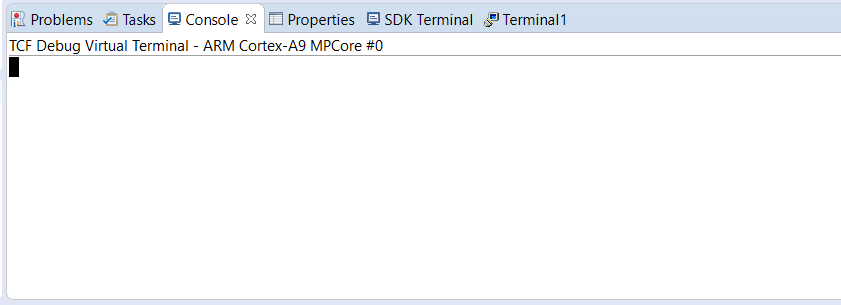
\includegraphics[width=1\columnwidth]{Images/terminal.png}
    \caption{SDK Terminal après avoir exécuté le code}
\end{figure}

\subsection{Utilisation des Ressources}

Vivado génère un rapport détaillé de la synthèse matériel, qui inclut :
\begin{itemize}
    \item Les \textbf{LUTs} (Look-Up Tables) utilisées, en pourcentage du total disponible.
    \item La mémoire \textbf{BRAM} (Block RAM) utilisée.
    \item Les \textbf{DSP Slices} (Digital Signal Processing) exploitées pour accélérer les calculs mathématiques complexes.
\end{itemize}

Ces informations nous permettent d'optimiser la conception tout en assurant que les ressources disponibles sur le FPGA ne sont pas épuisées.

Les données collectées sur le temps d'exécution et l'utilisation des ressources pour différentes configurations nous permettent de tracer les courbes de performance :
\begin{itemize}
    \item \textbf{Courbes de latence} : montrent le temps d'exécution en fonction des configurations.
    \item \textbf{Courbes de Pareto} : illustrent le compromis entre la réduction du temps d'exécution et l'augmentation de l'utilisation des ressources.
\end{itemize}


La \textbf{frontière de Pareto} est essentielle pour optimiser notre système. Elle montre qu'il est difficile d'améliorer une métrique (comme la latence) sans aggraver une autre (comme l'utilisation des ressources). Nos résultats devraient suivre cette logique.

\subsection{Optimisations Potentielles}

Pour améliorer les performances du système, plusieurs optimisations peuvent être appliquées :
\begin{itemize}
    \item \textbf{Unrolling} : permet d'exécuter plusieurs itérations d'une boucle en parallèle, augmentant ainsi le parallélisme et réduisant la latence.
    \item \textbf{Pipelining} : permet aux différentes étapes d'un calcul de s'exécuter simultanément, améliorant ainsi le débit global.
    \item \textbf{Resource Sharing} : partage des ressources matérielles comme les DSP entre plusieurs opérations, ce qui réduit l'utilisation globale des ressources au prix d'une légère augmentation de la latence.
\end{itemize}

Ces stratégies d'optimisation sont cruciales pour maximiser l'efficacité du système tout en minimisant l'empreinte matérielle.

\end{document}
